%===============================================================================
% LaTeX sjabloon voor de bachelorproef toegepaste informatica aan HOGENT
% Meer info op https://github.com/HoGentTIN/latex-hogent-report
%===============================================================================

\documentclass[dutch,dit,thesis]{hogentreport}

% TODO:
% - If necessary, replace the option `dit`' with your own department!
%   Valid entries are dbo, dbt, dgz, dit, dlo, dog, dsa, soa
% - If you write your thesis in English (remark: only possible after getting
%   explicit approval!), remove the option "dutch," or replace with "english".

%%\usepackage{lipsum} % For blind text, can be removed after adding actual content

%% Pictures to include in the text can be put in the graphics/ folder
\graphicspath{{../graphics/}}

%% For source code highlighting, requires pygments to be installed
%% Compile with the -shell-escape flag!
\usepackage[chapter]{minted}
%% If you compile with the make_thesis.{bat,sh} script, use the following
%% import instead:
%% \usepackage[chapter,outputdir=../output]{minted}
\usemintedstyle{solarized-light}

%% Formatting for minted environments.
\setminted{%
    autogobble,
    frame=lines,
    breaklines,
    linenos,
    tabsize=4
}

%% Ensure the list of listings is in the table of contents
\renewcommand\listoflistingscaption{%
    \IfLanguageName{dutch}{Lijst van codefragmenten}{List of listings}
}
\renewcommand\listingscaption{%
    \IfLanguageName{dutch}{Codefragment}{Listing}
}
\renewcommand*\listoflistings{%
    \cleardoublepage\phantomsection\addcontentsline{toc}{chapter}{\listoflistingscaption}%
    \listof{listing}{\listoflistingscaption}%
}

% Other packages not already included can be imported here

\usepackage{multirow,booktabs,setspace,caption}
\usepackage{tikz}

\DeclareCaptionLabelSeparator*{spaced}{\\[2ex]}
\captionsetup[table]{textfont=it,format=plain,justification=justified,
    singlelinecheck=false,labelsep=spaced,skip=0pt}
\captionsetup[figure]{labelsep=period,labelfont=it,justification=justified,
    singlelinecheck=false,font=doublespacing}

%%---------- Document metadata -------------------------------------------------
% TODO: Replace this with your own information
\author{Jan De Somviele}
\supervisor{Mevr. L. De Mol}
\cosupervisor{Mevr. G. Vercauteren}
\title[]%
    {De impact van mobiele netwerken op facilitair beheer: een vergelijkende studie van 4G en privaat 5G voor HOGENT}
\academicyear{\advance\year by -1 \the\year--\advance\year by 1 \the\year}
\examperiod{2}
\degreesought{\IfLanguageName{dutch}{Professionele bachelor in de toegepaste informatica}{Bachelor of applied computer science}}
\partialthesis{false} %% To display 'in partial fulfilment'
%\institution{Internshipcompany BVBA.}

%% Add global exceptions to the hyphenation here
\hyphenation{back-slash}

%% The bibliography (style and settings are  found in hogentthesis.cls)
\addbibresource{bachproef.bib}            %% Bibliography file
\addbibresource{../voorstel/voorstel.bib} %% Bibliography research proposal
\defbibheading{bibempty}{}

%% Prevent empty pages for right-handed chapter starts in twoside mode
\renewcommand{\cleardoublepage}{\clearpage}

\renewcommand{\arraystretch}{1.2}

%% Content starts here.
\begin{document}

%---------- Front matter -------------------------------------------------------

\frontmatter

\hypersetup{pageanchor=false} %% Disable page numbering references
%% Render a Dutch outer title page if the main language is English
\IfLanguageName{english}{%
    %% If necessary, information can be changed here
    \degreesought{Professionele Bachelor toegepaste informatica}%
    \begin{otherlanguage}{dutch}%
       \maketitle%
    \end{otherlanguage}%
}{}

%% Generates title page content
\maketitle
\hypersetup{pageanchor=true}

%%=============================================================================
%% Voorwoord
%%=============================================================================

\chapter*{\IfLanguageName{dutch}{Woord vooraf}{Preface}}%
\label{ch:voorwoord}

%% TODO:
%% Het voorwoord is het enige deel van de bachelorproef waar je vanuit je
%% eigen standpunt (``ik-vorm'') mag schrijven. Je kan hier bv. motiveren
%% waarom jij het onderwerp wil bespreken.
%% Vergeet ook niet te bedanken wie je geholpen/gesteund/... heeft

\lipsum[1-2]
%%=============================================================================
%% Samenvatting
%%=============================================================================

% TODO: De "abstract" of samenvatting is een kernachtige (~ 1 blz. voor een
% thesis) synthese van het document.
%
% Een goede abstract biedt een kernachtig antwoord op volgende vragen:
%
% 1. Waarover gaat de bachelorproef?
% 2. Waarom heb je er over geschreven?
% 3. Hoe heb je het onderzoek uitgevoerd?
% 4. Wat waren de resultaten? Wat blijkt uit je onderzoek?
% 5. Wat betekenen je resultaten? Wat is de relevantie voor het werkveld?
%
% Daarom bestaat een abstract uit volgende componenten:
%
% - inleiding + kaderen thema
% - probleemstelling
% - (centrale) onderzoeksvraag
% - onderzoeksdoelstelling
% - methodologie
% - resultaten (beperk tot de belangrijkste, relevant voor de onderzoeksvraag)
% - conclusies, aanbevelingen, beperkingen
%
% LET OP! Een samenvatting is GEEN voorwoord!

%%---------- Nederlandse samenvatting -----------------------------------------
%
% TODO: Als je je bachelorproef in het Engels schrijft, moet je eerst een
% Nederlandse samenvatting invoegen. Haal daarvoor onderstaande code uit
% commentaar.
% Wie zijn bachelorproef in het Nederlands schrijft, kan dit negeren, de inhoud
% wordt niet in het document ingevoegd.

\IfLanguageName{english}{%
\selectlanguage{dutch}
\chapter*{Samenvatting}
\lipsum[1-4]
\selectlanguage{english}
}{}

%%---------- Samenvatting -----------------------------------------------------
% De samenvatting in de hoofdtaal van het document

\chapter*{\IfLanguageName{dutch}{Samenvatting}{Abstract}}

\lipsum[1-4]


%---------- Inhoud, lijst figuren, ... -----------------------------------------

\tableofcontents

% In a list of figures, the complete caption will be included. To prevent this,
% ALWAYS add a short description in the caption!
%
%  \caption[short description]{elaborate description}
%
% If you do, only the short description will be used in the list of figures

\listoffigures

% If you included tables and/or source code listings, uncomment the appropriate
% lines.
\listoftables

%\listoflistings

% Als je een lijst van afkortingen of termen wil toevoegen, dan hoort die
% hier thuis. Gebruik bijvoorbeeld de ``glossaries'' package.
% https://www.overleaf.com/learn/latex/Glossaries

%---------- Kern ---------------------------------------------------------------

\mainmatter{}

% De eerste hoofdstukken van een bachelorproef zijn meestal een inleiding op
% het onderwerp, literatuurstudie en verantwoording methodologie.
% Aarzel niet om een meer beschrijvende titel aan deze hoofdstukken te geven of
% om bijvoorbeeld de inleiding en/of stand van zaken over meerdere hoofdstukken
% te verspreiden!
%%=============================================================================
%% Inleiding
%%=============================================================================

\chapter{\IfLanguageName{dutch}{Inleiding}{Introduction}}%
\label{ch:inleiding}

Deze bachelorproef richt zich op het onderzoeken van de impact van de overstap van een bekabeld netwerk naar mobiele netwerken, zoals 4G, privaat 5G, en publiek 5G, voor de facilitaire diensten verwarming en verlichting van HOGENT. Doordat apparatuur steeds meer gebruik maakt van internettoegang en cloudmanagement, wordt de vraag gesteld of een mobiel netwerk een een betrouwbare en veilige oplossing kan bieden. Momenteel worden verlichting en verwarming op de campus Schoonmeersen geautomatiseerd aangestuurd via tijdschema's, sensoren en regelmodules. De overstap naar een mobiel netwerk brengt zowel voordelen als uitdagingen mee: een mobiel netwerk belooft snellere verbindingen en flexibiliteit, maar zorgt ook voor de nood aan afwegingen met betrekking tot bandbreedte, netwerkbelasting en veiligheid. De doelgroep van dit onderzoek is het faciliteir beheer van HOGENT. De centrale onderzoeksvraag van deze bachelorproef is: \textit{Welk netwerk (4G, privaat 5G of publiek 5G) biedt de beste balans tussen beveiliging, prestaties en netwerkbelasting voor de facilitaire diensten verwarming en verlichting van HOGENT?}. Naast deze onderzoeksvraag worden volgende vragen ook beantwoord: 
\begin{itemize}
    \item Welke technische vereisten hebben de systemen voor verwarming en verlichting op HOGENT-locaties?
    \item Wat zijn de veiligheidsrisico’s bij het gebruik van mobiele netwerken voor verwarming en verlichting, en hoe kunnen deze worden beperkt?
    \item Welke aanpassingen zijn nodig om de bestaande bekabelde systemen voor verwarming en verlichting compatibel te maken met mobiele netwerken?
    \item Wat zijn de implicaties van de keuze voor een mobiel netwerk op de operationele continuïteit van de diensten verwarming en verlichting?
    \item Wat zijn de implicaties van een overstap naar een mobiel netwerk voor onderhoud en beheer van de verwarmings- en verlichtingssystemen?
    \item Is het zinvol om volledig over te stappen naar een privaat 5G netwerk, en hoe kan dit het best worden gerealiseerd?
\end{itemize}
%
%De inleiding moet de lezer net genoeg informatie verschaffen om het onderwerp te begrijpen en in te zien waarom de onderzoeksvraag de moeite waard is om te onderzoeken. In de inleiding ga je literatuurverwijzingen beperken, zodat de tekst vlot leesbaar blijft. Je kan de inleiding verder onderverdelen in secties als dit de tekst verduidelijkt. Zaken die aan bod kunnen komen in de inleiding~\autocite{Pollefliet2011}:
%
%\begin{itemize}
%  \item context, achtergrond
%  \item afbakenen van het onderwerp
%  \item verantwoording van het onderwerp, methodologie
%  \item probleemstelling
%  \item onderzoeksdoelstelling
%  \item onderzoeksvraag
%  \item \ldots
%\end{itemize}
%
%\section{\IfLanguageName{dutch}{Probleemstelling}{Problem Statement}}%
%\label{sec:probleemstelling}
%
%Uit je probleemstelling moet duidelijk zijn dat je onderzoek een meerwaarde heeft voor een concrete doelgroep. De doelgroep moet goed gedefinieerd en afgelijnd zijn. Doelgroepen als ``bedrijven,'' ``KMO's'', systeembeheerders, enz.~zijn nog te vaag. Als je een lijstje kan maken van de personen/organisaties die een meerwaarde zullen vinden in deze bachelorproef (dit is eigenlijk je steekproefkader), dan is dat een indicatie dat de doelgroep goed gedefinieerd is. Dit kan een enkel bedrijf zijn of zelfs één persoon (je co-promotor/opdrachtgever).
%
%\section{\IfLanguageName{dutch}{Onderzoeksvraag}{Research question}}%
%\label{sec:onderzoeksvraag}
%
%Wees zo concreet mogelijk bij het formuleren van je onderzoeksvraag. Een onderzoeksvraag is trouwens iets waar nog niemand op dit moment een antwoord heeft (voor zover je kan nagaan). Het opzoeken van bestaande informatie (bv. ``welke tools bestaan er voor deze toepassing?'') is dus geen onderzoeksvraag. Je kan de onderzoeksvraag verder specifiëren in deelvragen. Bv.~als je onderzoek gaat over performantiemetingen, dan 
%
%\section{\IfLanguageName{dutch}{Onderzoeksdoelstelling}{Research objective}}%
%\label{sec:onderzoeksdoelstelling}
%
%Wat is het beoogde resultaat van je bachelorproef? Wat zijn de criteria voor succes? Beschrijf die zo concreet mogelijk. Gaat het bv.\ om een proof-of-concept, een prototype, een verslag met aanbevelingen, een vergelijkende studie, enz.

\section{\IfLanguageName{dutch}{Opzet van deze bachelorproef}{Structure of this bachelor thesis}}%
\label{sec:opzet-bachelorproef}

% Het is gebruikelijk aan het einde van de inleiding een overzicht te
% geven van de opbouw van de rest van de tekst. Deze sectie bevat al een aanzet
% die je kan aanvullen/aanpassen in functie van je eigen tekst.

De rest van deze bachelorproef is als volgt opgebouwd:

In Hoofdstuk~\ref{ch:stand-van-zaken} wordt een overzicht gegeven van de stand van zaken binnen het onderzoeksdomein, op basis van een literatuurstudie.

In Hoofdstuk~\ref{ch:methodologie} wordt de methodologie toegelicht en worden de gebruikte onderzoekstechnieken besproken om een antwoord te kunnen formuleren op de onderzoeksvragen.

% TODO: Vul hier aan voor je eigen hoofstukken, één of twee zinnen per hoofdstuk

In Hoofdstuk~\ref{ch:scripts} wordt de gebruikte scripts uitgelegd.
In Hoofdstuk~\ref{ch:basisopstelling} wordt de eerste opstelling voor de testen uitgelegd.
In Hoofdstuk~\ref{ch:uitgebreide-opstelling} wordt de uitgebreide opstelling uitgelegd.
In Hoofdstuk~\ref{ch:resultaten} worden de resultaten van de testen uitgelegd.

In Hoofdstuk~\ref{ch:conclusie}, tenslotte, wordt de conclusie gegeven en een antwoord geformuleerd op de onderzoeksvragen. Daarbij wordt ook een aanzet gegeven voor toekomstig onderzoek binnen dit domein.
\chapter{\IfLanguageName{dutch}{Stand van zaken}{State of the art}}%
\label{ch:stand-van-zaken}

% Tip: Begin elk hoofdstuk met een paragraaf inleiding die beschrijft hoe
% dit hoofdstuk past binnen het geheel van de bachelorproef. Geef in het
% bijzonder aan wat de link is met het vorige en volgende hoofdstuk.

% Pas na deze inleidende paragraaf komt de eerste sectiehoofding.
\section{Inleiding}

%Dit hoofdstuk bevat je literatuurstudie. De inhoud gaat verder op de inleiding, maar zal het onderwerp van de bachelorproef *diepgaand* uitspitten. De bedoeling is dat de lezer na lezing van dit hoofdstuk helemaal op de hoogte is van de huidige stand van zaken in het onderzoeksdomein. Iemand die niet vertrouwd is met het onderwerp, weet nu voldoende om de rest van het verhaal te kunnen volgen, zonder dat die er nog andere informatie moet over opzoeken \autocite{Pollefliet2011}.
%
%Je verwijst bij elke bewering die je doet, vakterm die je introduceert, enz.\ naar je bronnen. In \LaTeX{} kan dat met het commando \texttt{$\backslash${textcite\{\}}} of \texttt{$\backslash${autocite\{\}}}. Als argument van het commando geef je de ``sleutel'' van een ``record'' in een bibliografische databank in het Bib\LaTeX{}-formaat (een tekstbestand). Als je expliciet naar de auteur verwijst in de zin (narratieve referentie), gebruik je \texttt{$\backslash${}textcite\{\}}. Soms is de auteursnaam niet expliciet een onderdeel van de zin, dan gebruik je \texttt{$\backslash${}autocite\{\}} (referentie tussen haakjes). Dit gebruik je bv.~bij een citaat, of om in het bijschrift van een overgenomen afbeelding, broncode, tabel, enz. te verwijzen naar de bron. In de volgende paragraaf een voorbeeld van elk.
%
%\textcite{Knuth1998} schreef een van de standaardwerken over sorteer- en zoekalgoritmen. Experten zijn het erover eens dat cloud computing een interessante opportuniteit vormen, zowel voor gebruikers als voor dienstverleners op vlak van informatietechnologie~\autocite{Creeger2009}.
%
%Let er ook op: het \texttt{cite}-commando voor de punt, dus binnen de zin. Je verwijst meteen naar een bron in de eerste zin die erop gebaseerd is, dus niet pas op het einde van een paragraaf.
%
%\begin{figure}
%  \centering
%  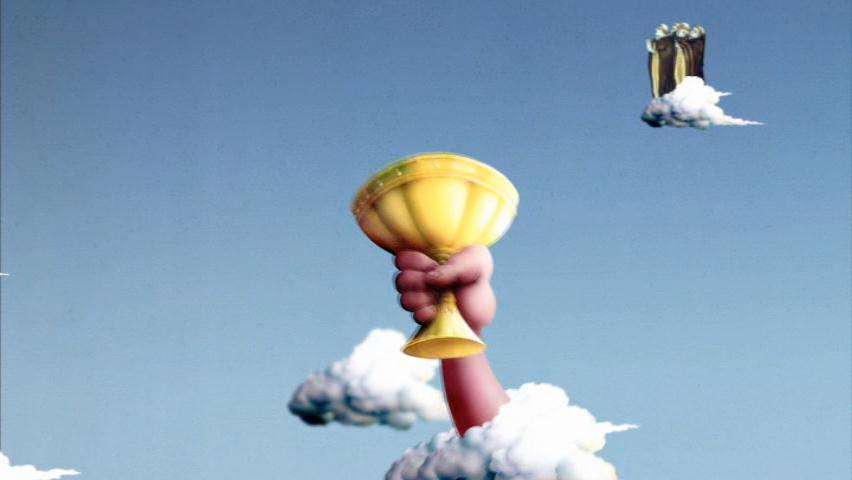
\includegraphics[width=0.8\textwidth]{grail.jpg}
%  \caption[Voorbeeld figuur.]{\label{fig:grail}Voorbeeld van invoegen van een figuur. Zorg altijd voor een uitgebreid bijschrift dat de figuur volledig beschrijft zonder in de tekst te moeten gaan zoeken. Vergeet ook je bronvermelding niet!}
%\end{figure}

%\begin{listing}
%  \begin{minted}{txt}
%    import pandas as pd
%    import seaborn as sns
%
%    penguins = sns.load_dataset('penguins')
%    sns.relplot(data=penguins, x="flipper_length_mm", y="bill_length_mm", hue="species")
%  \end{minted}
%  \caption[Voorbeeld codefragment]{Voorbeeld van het invoegen van een codefragment.}
%\end{listing}

%\lipsum[7-20]

%\begin{table}
%  \centering
%  \begin{tabular}{lcr}
%    \toprule
%    \textbf{Kolom 1} & \textbf{Kolom 2} & \textbf{Kolom 3} \\
%    $\alpha$         & $\beta$          & $\gamma$         \\
%    \midrule
%    A                & 10.230           & a                \\
%    B                & 45.678           & b                \\
%    C                & 99.987           & c                \\
%    \bottomrule
%  \end{tabular}
%  \caption[Voorbeeld tabel]{\label{tab:example}Voorbeeld van een tabel.}
%\end{table}
\section{Facilitair beheer}
Facilitair beheer (FM) is een interdisciplinair vakgebied dat de coördinatie van mensen, processen en ruimtes omvat om welzijn en efficiëntie binnen organisaties te verbeteren (ISO 41011:2018) \autocite{jaouhari2023we}. 

\section{facilitaire diensten van HOGENT}
Het centrale punt voor het beheer van facilitaire diensten op HOGENT heeft als locatie de campus Mercator. Hier wordt de informatie verzameld en gemonitord van alle campusen binnen het gebouwbeheersysteem. Voor deze bachelorproef wordt er dieper ingegaan op de campus Schoonmeersen.

\subsection{Campus Schoonmeersen}
Op de campus Schoonmeersen zijn er 2 platformen om de informatie te verzamelen van de facilitaire diensten. Deze platformen zijn Johnson controls Metasys en Schneider's Schneider Electric. Metasys is in gebruik in gebouw D (GSCHD) zie figuur 2.1 en Scneider Electric is in gebruik in de gebouwen B (GSCHB), C (GSCHC), P (GSCHP) en de HOGENT Sporthal zie figuur 2.2 \autocite{Venneman2019}.

\begin{figure}
    \centering
    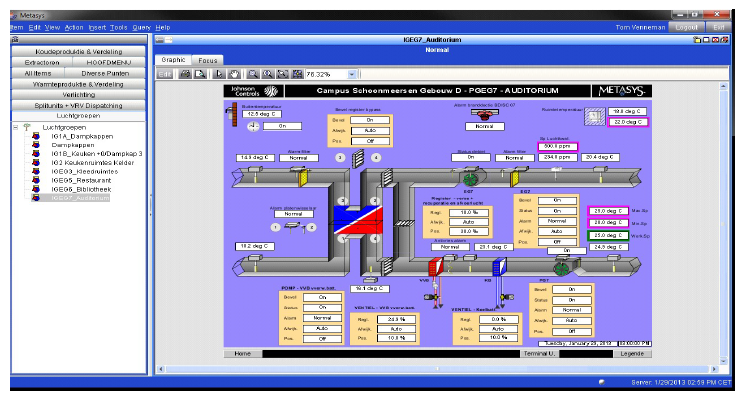
\includegraphics[width=0.8\textwidth]{metasys.png}
    \caption[metasys bron. HOGENT gebouwbeheersysteem (Metasys)]{\label{fig:metasys}metasys bron. HOGENT gebouwbeheersysteem (Metasys), luchtgroep gebouw D}
\end{figure}
\begin{figure}
    \centering
    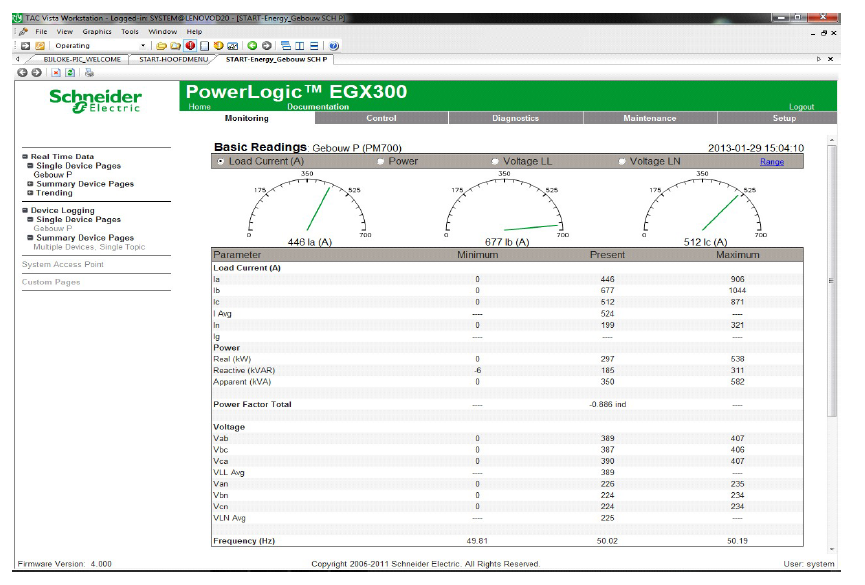
\includegraphics[width=0.8\textwidth]{Schneider_Electric.png}
    \caption[Schneider Electric. bron. HOGENT gebouwbeheersysteem (Schneider Electric)]{\label{fig:schneiderelectric}Schneider Electric. bron. HOGENT gebouwbeheersysteem (Schneider Electric), weergave van het stroom- en spanningsverbruik en het vermogen van het gebouw P op de campus Schoonmeersen.}
\end{figure}

\subsection{Xenta modules}
In de gebouwen wordt er gebruik gemaakt van Xenta modules. Xenta module 401 is telkens de hoofdregelaar voor de systemen. Hieraan zijn dan telkens maximaal 10 input output apparaten verbonden en deze staan dan in voor het verzamelen van de gegevens van de diverse metingen. Er zijn verschillende soorten van input output apparaten zoals te zien in figuur 2.3. Digitale input en output apparaten hebben 2 vaste staten zoals uit en aan. Een thermistor is een weerstandsthermometer, of een resistor waarvan de weerstand afhankelijk is van de temperatuur. Analoge apparaten gebruiken continue signalen die variëren in grootte, zoals spanning, stroom of weerstand. Universele apparaten zijn apparaten die zowel kunnen dienen als digitale input en output en als analoge output.

\begin{figure}
  \centering
  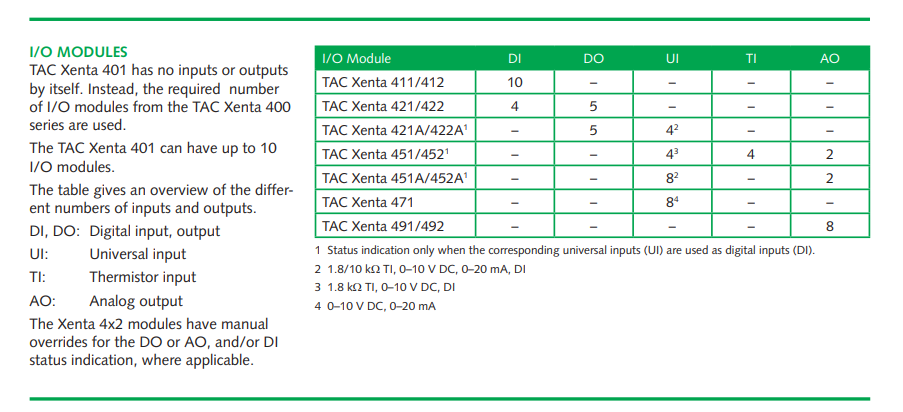
\includegraphics[width=0.8\textwidth]{tabel_XentaModules.png}
  \caption[Xenta modules. bron. Schneider Electric documenten]{\label{fig:xentamodules}Xenta modules. bron. Schneider Electric documenten}
\end{figure}


%\subsection{Spacelogic}
%De gebouwen op de campus Schoonmeersen maken gebruik van een Spacelogic controller AS-P om te communiceren via een toegewezen ip adres.

% TO DO: foto's bijzetten
\subsection{Verlichting}
Op het hoofdscherm van het systeem bevindt zich een schakelaar waarmee de verlichting van de gebouwen vanuit Mercator kan worden aangestuurd. De verlichting werkt volgens een vooraf ingesteld tijdschema. Binnen de gebouwen mogen de lichten aanstaan op de volgende tijden:

\begin{itemize}
    \item \textbf{Maandag tot en met vrijdag:} 05:30 -- 22:00
    \item \textbf{Zaterdag:} 07:00 -- 19:00
\end{itemize}

Voor de buitenverlichting geldt een iets ruimer tijdschema:

\begin{itemize}
    \item \textbf{Maandag tot en met vrijdag:} 05:30 -- 22:15
    \item \textbf{Zaterdag:} 07:20 -- 19:20
\end{itemize}

Naast tijdsinstellingen wordt ook de helderheid gemeten om te bepalen of verlichting noodzakelijk is. Voor binnenverlichting geldt een drempelwaarde van $60.000$ lux, terwijl deze voor buitenverlichting op $60$ lux ligt. Wanneer de helderheid onder deze grenswaarden komt, kan de verlichting worden ingeschakeld.

Voor gebouwen waarbij de verlichting niet vanuit Mercator kan worden aangestuurd, gebeurt de bediening handmatig.

\subsection{HVAC (Heating, Ventilation, and Air Conditioning)}
Gebouw T beschikt over het meest geavanceerde HVAC-systeem op de campus Schoonmeersen en dient als referentie voor de overige gebouwen. De warmteproductie binnen de gebouwen wordt voornamelijk verzorgd door ketels. In Gebouw T is daarnaast een warmtepomp geïnstalleerd, wat zorgt voor een efficiëntere en flexibelere regeling.

De werking van de ketels is gebaseerd op het aantal draaiuren, wat vooral van belang is voor onderhoudsplanning. Wanneer een warmtepomp aanwezig is, fungeert deze als \textbf{primaire} warmtebron, terwijl de ketels als \textbf{secundaire} warmtevoorziening dienen.

De warmtepomp hanteert specifieke temperatuursinstellingen:

\begin{itemize}
    \item \textbf{Verwarming (heating):} Ingeschakeld bij een temperatuur onder $16^{\circ}C$
    \item \textbf{Neutrale stand:} Tussen $16^{\circ}C$ en $18^{\circ}C$
    \item \textbf{Koeling (cooling):} Geactiveerd bij temperaturen boven $18^{\circ}C$
    \item \textbf{Vorstbescherming:} In de winter schakelt het systeem automatisch over op verwarming wanneer de temperatuur onder $5^{\circ}C$ daalt
\end{itemize}

\subsubsection{Zone-indeling en temperatuurregeling}
De gebouwen zijn opgedeeld in verschillende verwarmingskringen, waarbij een kring een verzameling radiatoren omvat. In oudere gebouwen vormen deze kringen het eindpunt van de regeling, terwijl Gebouw T daarnaast nog extra \textbf{zoneregelaars} per lokaal heeft. Hierdoor is een meer gedetailleerde temperatuurregeling mogelijk.

De verwarmingskringen werken volgens een \textbf{tijdsschema}:

\begin{itemize}
    \item \textbf{Maandag tot en met zaterdag:} 05:30 -- 17:30
    \item \textbf{Donderdag:} Uitgebreide werking tot 19:30
    \item \textbf{Nachttemperatuur:} 16$^{\circ}$C
    \item \textbf{Overdag:} De binnenruimtetemperatuur wordt automatisch aangepast op basis van de buitentemperatuur, met een gemiddelde richtwaarde van 19$^{\circ}$C
\end{itemize}

Dankzij de zoneregelaars kan de temperatuur per lokaal worden aangepast. Hierbij wordt rekening gehouden met aanwezigheidssensoren die de ruimtestatus bepalen:

\begin{itemize}
    \item \textbf{Unoccupied:} Ruimte is niet in gebruik $\rightarrow$ 16$^{\circ}$C
    \item \textbf{Standby:} Ruimte is actief, maar leeg $\rightarrow$ 18$^{\circ}$C
    \item \textbf{Occupied:} Ruimte is in gebruik $\rightarrow$ 19$^{\circ}$C
\end{itemize}

\subsubsection{Ventilatie}
De ventilatie wordt geregeld per luchtgroep. Buitenlucht wordt via een warmtewiel en een warmtebatterij (kleine warmtekring) gefilterd en opgewarmd voordat het via ventilatoren naar binnen wordt gebracht. De ventilatie werkt op basis van zowel een tijdsklok als een \textbf{drukregeling}, waarbij de druk binnen de waarden van $400$ Pa tot $500$ Pa blijft.

In Gebouw T kunnen de zoneregelaars ook de ventilatie aansturen. Dit gebeurt op basis van \textbf{CO$_2$-concentratie}. Wanneer de CO$_2$-waarde de drempel van $800$ ppm overschrijdt, worden de regelkleppen automatisch meer geopend om extra ventilatie toe te laten.

Elk van deze regelmodules verzamelt en logt verschillende meetwaarden, waardoor temperatuur- en ventilatiegegevens grafisch kunnen worden weergegeven.

\subsubsection{Verwarmingsperiode}
Het stookseizoen loopt doorgaans van \textbf{oktober tot april/mei}, afhankelijk van de buitentemperaturen en de verwarmingsbehoefte.

\subsection{Storingen en Monitoring}
Storingen worden in \textbf{realtime} geregistreerd en weergegeven in Mercator via een overzichtelijke lijst. Hierdoor kunnen bekende problemen direct worden gemonitord en kunnen storingen snel worden opgelost voordat ze een impact hebben op het comfort binnen de gebouwen.

\section{Vergelijking 4G en 5G}
Het verschil tussen 4G en 5G in facilitair beheer ligt in de infrastructuur en middelenbeheer. 5G biedt flexibelere en efficiëntere infrastructuur dankzij virtualisatie wat zorgt voor schaalbaarheid en minder handmatige interventie \autocite{degambur2021resource}. 5G introduceert een verbeterde netwerkcapaciteit, betrouwbaarheid en efficiëntie, met lagere latentie en lager energieverbruik ten opzichte van 4G. De nadruk ligt op hoge snelheden en het verbinden van meerdere apparaten tegelijkertijd \autocite{mihret20214g}. De integratie van 5G technologie in het facilitair beheer van slimme gebouwen biedt voordelen voor efficiëntie, connectiviteit en veiligheid. Hoewel uitdagingen zoals hoge investeringskosten en complexe integratie bestaan, maar de voordelen van verbeterde duurzaamheid, efficiëntie en comfort overtreffen deze uitdagingen \autocite{Markogiannaki2023}. Private 5G netwerken bieden bedrijven en organisaties een veilig, flexibel en schaalbaar alternatief voor publieke 5G netwerken. Private 5G netwerken maken het mogelijk om data veilig en autonoom te delen zonder de openbare internetinfrastructuur te gebruiken \autocite{eswaran2023private}.

5G biedt hogere datasnelheden, lagere latentie en ondersteuning voor veel meer verbonden apparaten  dan 4G dankzij mmWave-technologie, massive MIMO en ultra-dense netwerken \autocite{Hui_2020}.


\section{Smart campussen}
\textcites{Min_Allah_2020,AbuAlnaaj2016,Ahmed2022} beschrijven hoe smart campussen geavanceerde technologieën zoals het Internet of Things (IoT), 5G-connectiviteit en kunstmatige intelligentie (AI) gebruiken om onderwijsinstellingen efficiënter, duurzamer en gebruiksvriendelijker te maken. Deze technologieën verbeteren niet alleen de leeromgeving, maar optimaliseren ook energiebeheer, beveiliging en operationele efficiëntie \autocite{Correia2022}. Een belangrijke uitdaging bij de implementatie van smart campus-technologieën is de hoge kosten, cyberveiligheidsrisico’s en de noodzaak van een geïntegreerde infrastructuur \autocite{Liu_2022}. Desondanks tonen studies aan dat de voordelen, zoals energiebesparing en verhoogde veiligheid, opwegen tegen deze uitdagingen \autocite{AbuAlnaaj2016}.

\section{IoT en 5G in smart campussen, steden en gebouwen}

\textcite{Bilardo_2021} stelt dat IoT en 5G een cruciale rol spelen in de ontwikkeling van slimme steden en campussen door real-time monitoring en communicatie tussen apparaten mogelijk te maken. Hierdoor kunnen systemen zoals verlichting, klimaatregeling en beveiliging automatisch worden aangepast aan de behoeften van gebruikers, wat leidt tot een efficiënter energiegebruik en lagere operationele kosten \autocite{Polin2023}. De integratie van IoT binnen smart cities bevordert niet alleen duurzaamheidsdoelstellingen, maar verbetert ook de kwaliteit van leven door slimmere mobiliteit en infrastructuur \autocite{Chew2020}. Toch brengt de implementatie van IoT beveiligingsrisico’s met zich mee, zoals gegevenslekken en cyberaanvallen, wat een belangrijk aandachtspunt blijft voor beleidsmakers en technologieleveranciers \autocite{Trivedi2017}.

\section{HVAC-systemen en slim energiebeheer}

\textcite{Correia2022} legt uit dat efficiënte HVAC-systemen (verwarming, ventilatie en airconditioning) essentieel zijn voor slimme gebouwen en campussen, aangezien ze verantwoordelijk zijn voor een groot deel van het energieverbruik. Door AI en IoT te combineren, kunnen deze systemen worden geoptimaliseerd om energie te besparen zonder dat dit ten koste gaat van het comfort van gebruikers \autocite{Min_Allah_2020}. Geavanceerde algoritmes en machine learning spelen een grote rol bij het voorspellen van energieverbruik en het automatisch aanpassen van HVAC-instellingen om piekbelasting te verminderen \autocite{Khoa2020}. Daarnaast helpt IoT-technologie bij het continu monitoren en onderhouden van HVAC-systemen, waardoor storingen en inefficiëntie sneller kunnen worden opgespoord en verholpen \autocite{Zhang2022}.

\section{Slimme verlichting}

\textcite{Poyyamozhi2024} stelt dat slimme verlichting in zowel binnen- als buitenomgevingen bijdraagt aan energie-efficiëntie en verhoogd gebruikerscomfort. In gebouwen maken slimme verlichtingssystemen gebruik van sensoren en AI om de lichtsterkte en kleurtemperatuur aan te passen op basis van de aanwezigheid van personen en de hoeveelheid natuurlijk licht \autocite{Wang2024}. In buitenomgevingen, zoals smart cities, helpt geautomatiseerde straatverlichting energie te besparen door middel van bewegingsdetectie en connectiviteit met andere stadsnetwerken \autocite{Huseien_2022}. Hierdoor wordt niet alleen het energieverbruik verminderd, maar ook de veiligheid en bruikbaarheid van stedelijke ruimtes verbeterd.

Door de integratie van IoT, 5G en AI kunnen smart campussen en gebouwen op een duurzamere en efficiëntere manier functioneren. Hoewel er uitdagingen zijn zoals kosten en beveiligingsrisico’s, wegen de voordelen op lange termijn ruimschoots op tegen deze obstakels.







%%=============================================================================
%% Methodologie
%%=============================================================================

\chapter{\IfLanguageName{dutch}{Methodologie}{Methodology}}%
\label{ch:methodologie}

%% TODO: In dit hoofstuk geef je een korte toelichting over hoe je te werk bent
%% gegaan. Verdeel je onderzoek in grote fasen, en licht in elke fase toe wat
%% de doelstelling was, welke deliverables daar uit gekomen zijn, en welke
%% onderzoeksmethoden je daarbij toegepast hebt. Verantwoord waarom je
%% op deze manier te werk gegaan bent.
%% 
%% Voorbeelden van zulke fasen zijn: literatuurstudie, opstellen van een
%% requirements-analyse, opstellen long-list (bij vergelijkende studie),
%% selectie van geschikte tools (bij vergelijkende studie, "short-list"),
%% opzetten testopstelling/PoC, uitvoeren testen en verzamelen
%% van resultaten, analyse van resultaten, ...
%%
%% !!!!! LET OP !!!!!
%%
%% Het is uitdrukkelijk NIET de bedoeling dat je het grootste deel van de corpus
%% van je bachelorproef in dit hoofstuk verwerkt! Dit hoofdstuk is eerder een
%% kort overzicht van je plan van aanpak.
%%
%% Maak voor elke fase (behalve het literatuuronderzoek) een NIEUW HOOFDSTUK aan
%% en geef het een gepaste titel.

\section{Literatuuronderzoek en probleemdefinitie}

Het onderzoek startte met een literatuurstudie over 5G netwerken, smart gebouwen/campussen en de technische kenmerken, toepassingen en beperkingen van mobiele netwerken (4G, privaat 5G en wifi) in het kader van gebouwbeheersystemen. Er werd aandacht besteed aan latentie, bandbreedte en betrouwbaarheid binnen elk netwerktype. Parallel werd ook onderzocht hoe deze eigenschappen zich verhouden tot de vereisten van toepassingen zoals verlichting en HVAC, en wat de impact kan zijn op operationele stabiliteit.
Daarnaast werden gesprekken gevoerd met personeel van de directies IT- en facilitair beheer van HOGENT om inzicht te krijgen in de huidige architectuur, gebruikte protocollen , en gevoeligheden rond beveiliging en uptime van de gebouwenbeheerinfrastructuur. Deze fase resulteerde in een literatuurstudie en onderbouwing voor de testscenario’s.


\section{Ontwerp en realisatie van de testomgeving}

De testomgeving heeft als doel het gebouwbeheersysteem te simuleren. Omdat in HOGENT een fysieke SpaceLogic AS-P controller niet beschikbaar is voor experimentele doeleinden, wordt een alternatieve en flexibele testomgeving opgezet, gebaseerd op een Raspberry Pi 4 Model B. Deze microcomputer fungeert als centrale testnode en neemt de rol van edgecontroller op zich binnen de testopstelling. 
De keuze voor dit platform is gebaseerd op de brede ondersteuning van netwerkprotocollen, de programmeerbaarheid via Python en de mogelijkheid tot headless operaties en lokale datalogging. De Raspberry Pi voert daarbij zowel netwerkmetingen als simulaties van communicatie in gebouwbeheersystemen uit.
De Pi voert netwerktests uit met behulp van tools zoals ping, node-red, curl en iPerf3. Alle resultaten worden gelogd en bewaard om later te gebruiken.
Voor mobiele netwerkconnectiviteit wordt een industriële Teltonika RUTX50-router ingezet. Deze ondersteunt zowel 4G als 5G (zowel NSA als SA), en vormt de brug tussen de testnode en het externe netwerk. De combinatie van deze router met de Raspberry Pi maakt het mogelijk om in de verschillende netwerkomstandigheden metingen uit te voeren.
Een PC doet dienst als iperf3 TCP-server en simuleert een iperf server. Deze server reageert op de verzoeken van de Raspberry Pi, zodat dit een representatieve testomgeving creëert voor communicatie in een smart building-context.
De testomgeving omvat verschillende netwerken: wifi via een lokaal access point, privaat 4G en 5G via de RUTX50 router. Deze variatie biedt de mogelijkheid om met de testopstelling netwerkprestaties te vergelijken.
Deze opstelling vormt een goed alternatief voor fysieke gebouwbeheersysteem-hardware en is aldus geschikt voor experimenteel onderzoek naar IoT-communicatie binnen slimme gebouwen.


\section{Connectiviteits- en performantiemetingen}

In elk van de netwerkomgevingen wordt een identieke testreeks uitgevoerd. Het doel is om te evalueren hoe verschillende technologieën presteren op vlak van snelheid, betrouwbaarheid en stabiliteit.
De latency en jitter worden gemeten met behulp van het ping-commando . Voor de meting van throughput wordt gebruikgemaakt van zowel speedtest-cli, dat communiceert met publieke servers, als iPerf3, waarbij een eigen server op de pc fungeert als eindpunt.
Packet loss en stabiliteit worden geëvalueerd door langdurige communicatieopdrachten te herhalen. Zo voert de Raspberry Pi HTTP-verzoeken uit met curl naar een lokale Node-RED-server en registreert daarbij responstijden en eventuele fouten. 
Een extra test meet de reactietijd van een smart verlichting-toepassing. Via een lokaal netwerk wordt een Philips Hue-lamp twee keer geschakeld door een Python-script. De tijd tussen het commando en de feitelijke uitvoering wordt gelogd. Deze test illustreert concreet hoe netwerkomstandigheden de gebruikerservaring van een IoT-toepassing kunnen beïnvloeden.


\section{Uitvoer van de testscenario’s}

TO DO: uitleggen


\section{Data-analyse en evaluatie}

TO DO: anders
Alle verzamelde data wordt automatisch verwerkt met Python. De scripts analyseren latency, jitter, packet loss, doorvoersnelheden en systeembelasting. Deze gegevens worden omgezet naar visuele representaties zoals tijdreeksen, boxplots en gemiddeldevergelijkingen, wat helpt bij het identificeren van trends of anomalieën.
De evaluatie focust op prestatieverschillen tussen de onderzochte netwerktechnologieën - Wi-Fi, 4G en privaat 5G. Daarbij worden onder meer gemiddelde en maximale latency, jitterwaarden, en de frequentie van communicatieproblemen geanalyseerd. Ook wordt expliciet nagegaan hoe snel en betrouwbaar toepassingen reageren: van het schakelen van een lamp tot het succesvol polsen van Modbus-registers.
Naast deze kwantitatieve metingen wordt ook aandacht besteed aan operationele storingen of anomalieën zoals time-outs, verbindingsverlies of onverwacht gedrag tijdens de tests. Deze kwalitatieve observaties bieden inzicht in de betrouwbaarheid van de netwerken in dagelijkse toepassingen.









% Voeg hier je eigen hoofdstukken toe die de ``corpus'' van je bachelorproef
% vormen. De structuur en titels hangen af van je eigen onderzoek. Je kan bv.
% elke fase in je onderzoek in een apart hoofdstuk bespreken.

%\chapter{\IfLanguageName{dutch}{uitwerking}{}}%
\label{ch:uitweking}

%\chapter{\IfLanguageName{dutch}{scripts}{}}%
\label{ch:scripts}

\section*{Testscripts en validatie van de meetomgeving}

Om een objectieve vergelijking te kunnen maken tussen de prestaties van 4G- en 5G-netwerken in de context van gebouwbeheersystemen, werd er een reeks testscripts ontwikkeld in Python en Bash. Deze scripts dienen om op systematische wijze netwerkstatistieken te verzamelen, protocollaire communicatie te simuleren en de betrouwbaarheid van de verbinding tussen controlemodules en serveromgevingen te meten. In dit hoofdstuk wordt toegelicht welke scripts werden opgesteld, wat hun doel is binnen de testopstelling, hoe ze werken en hoe ze initieel gevalideerd werden op een lokaal wifinetwerk.

\section{Overzicht van de scripts}

De scripts zijn opgedeeld in twee hoofdcategorieën: netwerkdiagnose en protocolsimulatie.

\subsection*{Netwerkdiagnose (Bash-script)}

Het eerste script focust op algemene netwerkmetingen. Dit script voert periodiek ping-opdrachten uit naar de testrouter of controller en registreert daarbij de round-trip time (RTT), pakketverlies en jitter. Daarnaast worden iperf3-metingen uitgevoerd voor het analyseren van de beschikbare bandbreedte. De resultaten worden gelogd in een CSV-bestand voor latere analyse.

\textbf{Het script:}
% TO DO: script
%\begin{lstlisting}[language=bash]
%    #!/bin/bash
%    HOST="192.168.1.1"
%    LOG="ping_test.csv"
%    
%    echo "timestamp,rtt_min,rtt_avg,rtt_max,packet_loss" > $LOG
%    while true; do
%    OUT=$(ping -c 5 $HOST)
%    RTT=$(echo "$OUT" | tail -1 | awk -F '/' '{print $5","$6","$7}')
%    LOSS=$(echo "$OUT" | grep -oP '\d+(?=% packet loss)')
%    echo "$(date),$RTT,$LOSS" >> $LOG
%    sleep 60
%    done
%\end{lstlisting}

\subsection*{Modbus-communicatie test (Python-script)}

Het tweede script is gericht op het testen van industriële communicatie via het Modbus TCP-protocol. Dit script maakt gebruik van de \texttt{pymodbus}-bibliotheek om op geregelde tijdstippen waarden op te vragen bij een Xenta-module die met een AS-P controller verbonden is. Het meet de responstijd en controleert op fouten in de transmissie. Zo wordt nagegaan in welke mate netwerkvertragingen een impact hebben op de communicatie tussen veldmodules en beheersystemen.

\textbf{Het script:}
% TO DO: script
%\begin{lstlisting}[language=Python]
%    from pymodbus.client import ModbusTcpClient
%    import time, csv, datetime
%    
%    client = ModbusTcpClient('192.168.1.10', port=502)
%    with open("modbus_results.csv", "w", newline='') as file:
%    writer = csv.writer(file)
%    writer.writerow(["timestamp", "response_time_ms", "success"])
%    
%    while True:
%    start = time.time()
%    result = client.read_holding_registers(0, 1, unit=1)
%    end = time.time()
%    delta = round((end - start) * 1000, 2)
%    status = "OK" if result.isError() == False else "FAIL"
%    writer.writerow([datetime.datetime.now(), delta, status])
%    time.sleep(10)
%\end{lstlisting}

\section{Testdoelstellingen}

De scripts dienen meerdere doelen binnen de testopstelling:
\begin{itemize}
    \item Het verzamelen van relevante netwerkstatistieken, zoals latency, bandbreedte, jitter en pakketverlies.
    \item Het analyseren van de betrouwbaarheid van Modbus-communicatie over mobiele netwerken, wat representatief is voor het gedrag van HVAC- en verlichtingssystemen in realistische scenario’s.
    \item Het opsporen van storingen of onverwacht gedrag in de verbinding tussen modules via het mobiele netwerk.
    \item Het creëren van een reproduceerbare en geautomatiseerde testmethode voor consistente evaluaties.
\end{itemize}

\section{Eerste validatie op lokaal wifi-netwerk}

Voordat de scripts worden ingezet in de volledige testopstelling met 4G en 5G, worden ze eerst uitvoerig getest op het lokale wifi-netwerk. Deze validatiefase dient om mogelijke bugs in de scripts op te sporen, de logs te controleren op correcte structuur, en na te gaan of de scripts robuust functioneren bij langdurige uitvoering.

De gebruikte testomgeving bestond uit:
\begin{itemize}
    \item Een AS-P controller verbonden via ethernet met een router.
    \item Een PC of server verbonden via hetzelfde netwerk.
    \item De scripts werden uitgevoerd op de server die tegelijkertijd dienst deed als logger.
\end{itemize}

Tijdens deze validatiefase werd onder andere bevestigd dat:
\begin{itemize}
    \item De ping- en iperf3-metingen een correct verloop kenden en reproduceerbare resultaten gaven.
    \item De Modbus-simulatie foutloos opstartte, verbinding kon maken met de AS-P controller, en systematisch correcte registerwaarden ontving.
    \item CSV-bestanden correct en overzichtelijk werden opgebouwd voor latere verwerking in Excel of Python-analyse.
\end{itemize}

Deze validatiefase is van groot belang om zeker te zijn dat de scripts in latere fases waar netwerkverstoringen of bereikproblemen reëler zijn betrouwbaar blijven functioneren. Het beperkt de foutmarge en verhoogt de reproduceerbaarheid van de tests.

\chapter{\IfLanguageName{dutch}{basisopstelling}{basic set-up}}%
\label{ch:basisopstelling}

Om snel van start te kunnen gaan met het uitvoeren van testen en metingen werd een basisopstelling uitgewerkt waarbij geen gebruik wordt gemaakt van een externe server. Deze opstelling dient als eerste implementatie van het testnetwerk en biedt voldoende functionaliteit om al cruciale netwerkanalyses en communicatieproeven uit te voeren. In dit hoofdstuk wordt deze basisopstelling besproken, samen met de gebruikte componenten, verbindingen en de functionele doelen die hiermee gerealiseerd worden.

\section{Doel van de basisopstelling}

De bedoeling van deze initiële configuratie is om een minimale maar representatieve omgeving op te zetten waarin het gedrag van een gebouwbeheersysteem (GBS) getest kan worden over zowel een privaat 4G- als 5G-netwerk. De nadruk ligt hierbij op de communicatie tussen een Spacelogic AS-P controller en één of meerdere TAC Xenta-modules. Deze componenten vormen een realistische representatie van HVAC- en verlichtingssystemen in gebouwen.

Door het weglaten van een centrale server worden de scripts en logging lokaal uitgevoerd op een laptop of test-PC die direct met het netwerk verbonden is. Dit verlaagt de complexiteit van de opstartfase en maakt het eenvoudiger om foutopsporing te doen tijdens de eerste tests.

\section{Componenten in de opstelling}

De basisopstelling bevat de volgende kerncomponenten:
\begin{itemize}
    \item \textbf{Spacelogic AS-P Controller}: functioneert als centrale regelaar die via Modbus TCP communiceert met de Xenta-modules.
    \item \textbf{TAC Xenta Module (type 401)}: simulatie van een HVAC- of verlichtingsmodule die uitleesbaar is via Modbus.
    \item \textbf{Laptop of test-PC}: voert de testscripts uit en verzamelt meetgegevens (zoals latency, responstijden, packet loss, etc.).
    \item \textbf{Mobiel netwerk (4G of 5G)}: verbinding tussen de PC en de controller gebeurt via een mobiele router of gateway. Er wordt gebruikgemaakt van het privaat 4G/5G-netwerk beschikbaar op de HOGENT-campus.
\end{itemize}

\section{Verbindingsstructuur}
% TO DO: foto/de structuur kunnen tonen met dan uitleg eronder
De verbindingen worden als volgt gelegd:
\begin{enumerate}
    \item De AS-P controller wordt verbonden met een mobiele router/gateway via ethernet.
    \item De test-PC/laptop wordt via USB of ethernet verbonden met dezelfde mobiele router.
    \item De mobiele router is verbonden met het 4G- of 5G-netwerk, afhankelijk van het scenario.
    \item De TAC Xenta-module is bekabeld aangesloten op de AS-P controller via een RS-485-bus of IP, afhankelijk van de configuratie.
    \item Er is geen centrale server, dus alle scripts draaien op de test-PC.
\end{enumerate}

Deze opstelling maakt het mogelijk om onder reële netwerkcondities de communicatie en responstijd van het GBS te meten en zo de betrouwbaarheid van beide netwerken te evalueren.

\section{Functionele werking van de opstelling}

De communicatie tussen de PC en de controller wordt voortdurend gemonitord door de Python- en Bash-scripts die eerder besproken werden. Zo worden de volgende metingen uitgevoerd:
\begin{itemize}
    \item Latency tussen PC en controller via ping-tests.
    \item Bandbreedte en jitter via iperf3 indien ondersteund door de router.
    \item Realtime uitlezing van registers via Modbus TCP.
    \item Registratie van eventuele time-outs of fouten in de communicatie.
\end{itemize}

Alle meetresultaten worden gelogd en gestructureerd opgeslagen om later geanalyseerd te worden in functie van het gekozen netwerktype (4G of 5G).

\section{Voordelen van deze opstelling}
De voorgestelde opstelling biedt diverse voordelen die bijdragen aan een efficiënte en controleerbare testomgeving. Een belangrijk voordeel is de vereenvoudigde initiële opstart, aangezien er geen noodzaak bestaat tot het installeren of configureren van servers. Hierdoor wordt de implementatiedrempel aanzienlijk verlaagd. Bovendien vindt alle verwerking lokaal plaats op de testcomputer, wat directe controle en gedetailleerde logging mogelijk maakt. Dit bevordert de traceerbaarheid en vergemakkelijkt de foutanalyse.

Een ander essentieel voordeel betreft de duidelijke afbakening van het testdomein. Door het beperkt aantal betrokken variabelen kan de invloed van netwerkomstandigheden nauwkeuriger worden geïsoleerd en onderzocht. Tot slot is deze opstelling intrinsiek schaalbaar: indien uitbreiding gewenst is, kan een serversysteem zonder ingrijpende wijzigingen aan de bestaande structuur worden toegevoegd.
%\chapter{\IfLanguageName{dutch}{uitgebreide opstelling}{}}%
\label{ch:uitgebreide-opstelling}

Voor het uitvoeren van netwerkgerelateerde prestatietests op HVAC- en verlichtingssystemen in gebouw C, werd een testopstelling ontwikkeld waarin een private 4G- en 5G-netwerk vergeleken worden. Om deze tests op een gecontroleerde en schaalbare manier te kunnen uitvoeren, werd een kleine server opgenomen in het testnetwerk.

\section*{Doel van de opstelling}

Het hoofddoel van deze testopstelling is het evalueren van de performantie van communicatieprotocollen, zoals Modbus, die gebruikt worden voor het aansturen van TAC Xenta modules via een SpaceLogic AS-P controller. Er wordt onderzocht hoe deze systemen reageren onder verschillende netwerkcondities (4G vs 5G). De integratie van een lokale server maakt het mogelijk om testdata te genereren, netwerkverkeer te loggen en simulaties of scriptgestuurde polls uit te voeren.

\section*{Benodigde hardware}

\begin{itemize}
    \item \textbf{SpaceLogic AS-P controller} – fungeert als gateway tussen IP-netwerk en veldapparatuur (Modbus/RS485).
    \item \textbf{TAC Xenta modules (bv. Xenta 401)} – HVAC-controllers aangesloten via Modbus.
    \item \textbf{5G Router (bv. Teltonika RUTX50 of vergelijkbaar)} – verbindt de AS-P controller met het 5G netwerk.
    \item \textbf{4G Router} – voor testen over een privaat LTE-netwerk.
    \item \textbf{Mini Server (bv. Intel NUC of Raspberry Pi 5)} – draait scripts, verzamelt data en fungeert als testbedcontroller.
    \item \textbf{Laptop/PC} – voor initiële configuratie, monitoring en data-analyse.
    \item \textbf{Netwerkcomponenten} – Ethernetkabels, voeding, eventueel een switch.
\end{itemize}

\section*{Software en tools}

\begin{itemize}
    \item \textbf{Python/Bash scripts} – voor periodieke polling van Modbus registers en logging van reactietijden.
    \item \textbf{Grafana + InfluxDB} – voor visualisatie en opslag van netwerk- en systeemdata.
    \item \textbf{Tcpdump/iPerf} – netwerkdiagnosetools voor latency, jitter en packet loss.
    \item \textbf{Modbus client} – via Python (pymodbus) of modpoll CLI-tool.
\end{itemize}

\section*{Netwerkstructuur}

De server bevindt zich in hetzelfde subnet als de AS-P controller en is bereikbaar via zowel 4G als 5G afhankelijk van het testscenario. De Xenta modules zijn via Modbus (RTU of TCP) verbonden met de AS-P controller, die als interface naar het IP-netwerk fungeert. Alle communicatie tussen de controller en de server verloopt via de mobiele netwerken, waarbij testsoftware op de server de communicatie meet, logt en visualiseert.

\section*{Testprocedure}

\begin{enumerate}
    \item Configuratie van de AS-P: verbinding met Xenta modules opzetten, Modbus-mapping controleren.
    \item Netwerkconnectie testen: Router configureren voor respectievelijk 4G en 5G.
    \item Metingen uitvoeren:
    \begin{itemize}
        \item Latency: gemiddelde responstijd van Modbus polls.
        \item Jitter: variatie in responstijden.
        \item Packet loss: percentage verloren pakketten.
        \item Betrouwbaarheid: frequentie van time-outs of verbindingsonderbrekingen.
    \end{itemize}
    \item Data logging: met scripts wordt continu data opgeslagen op de server.
    \item Analyse \& vergelijking: met Grafana worden verschillen tussen 4G en 5G inzichtelijk gemaakt.
\end{enumerate}

\section*{Rol van de server}

De server speelt een centrale rol als controle- en dataverzamelpunt in de testopstelling. Het voordeel hiervan is dat alle meetdata lokaal opgeslagen kunnen worden, onafhankelijk van externe cloudverbindingen. Dit maakt reproduceerbare en betrouwbare metingen mogelijk en verlaagt de complexiteit van troubleshooting.



\chapter{\IfLanguageName{dutch}{resultaten}{results}}%
\label{ch:resultaten}

\section{Scripts}

\section{De opstelling}


%\input{...}
%\input{...}
%...

%%=============================================================================
%% Conclusie
%%=============================================================================

\chapter{Conclusie}%
\label{ch:conclusie}

% TODO: Trek een duidelijke conclusie, in de vorm van een antwoord op de
% onderzoeksvra(a)g(en). Wat was jouw bijdrage aan het onderzoeksdomein en
% hoe biedt dit meerwaarde aan het vakgebied/doelgroep? 
% Reflecteer kritisch over het resultaat. In Engelse teksten wordt deze sectie
% ``Discussion'' genoemd. Had je deze uitkomst verwacht? Zijn er zaken die nog
% niet duidelijk zijn?
% Heeft het onderzoek geleid tot nieuwe vragen die uitnodigen tot verder 
%onderzoek?



\section{Antwoord op de onderzoeksvraag}
Deze bachelorproef had als doel om te onderzoeken welk draadloos netwerk (4G of 5G) het meest geschikt is voor dataverkeer in een testomgeving waarin netwerkprestaties, lichtsturing en HTTP-verkeer via Node-RED centraal staan. Uit de uitgevoerde metingen en functionele testen blijkt dat elk netwerk verschillende sterktes vertoont, afhankelijk van de toepassing.
4G kwam naar voren als de meest stabiele en veelzijdige keuze voor toepassingen die betrouwbaarheid en continuïteit vereisen. Wifi biedt lage latency bij algemene netwerkcommunicatie, maar toonde zich minder stabiel bij functionele opdrachten zoals lichtsturing. 5G behaalt zeer hoge bandbreedte en snelle reacties bij functionele testen, maar kende ook grotere schommelingen in latency en jitter. Dit maakt 5G geschikt voor toepassingen met hoge datasnelheden, op voorwaarde dat de netwerkconfiguratie (bijvoorbeeld privaat 5G) een zekere voorspelbaarheid kan bieden.


\section{Bijdrage en meerwaarde voor het vakgebied}
De bijdrage van dit onderzoek ligt in het feit dat het niet alleen theoretische snelheden en latencies vergelijkt, maar die direct koppelt aan praktische use-cases. Door de combinatie van meetgegevens (iperf3, ping, packet captures) en functionele testen (lichtsturing, HTTP-verkeer) levert dit onderzoek bruikbare inzichten voor het toekomstige ontwerp van een gebouwbeheersysteem voor smart buildings.
In tegenstelling tot veel theoretische studies biedt dit werk voorbeelden van  praktisch, reproduceerbare scenario’s dicht aanleunen bij echte implementaties. De gebruikte methodologie vormt een nuttige basis voor toekomstig onderzoek of technische beslissingsondersteuning.


\section{Kritische reflectie en interpretatie van de resultaten}
In grote lijnen bevestigen de resultaten de verwachtingen: 5G biedt de hoogste prestaties op vlak van doorvoersnelheid, 4G is zeer betrouwbaar en wifi is snel maar gevoeliger voor verstoringen. Toch waren er ook onverwachte waarnemingen. Zo vertoonde 5G onverwacht hoge jitter- en latencypieken, wat wijst op onvoorspelbaarheid in publieke netwerken. Anderzijds was de reactietijd van 5G bij lichtsturing de snelste van de drie netwerken, wat aangeeft dat het voor lokale, kortstondige opdrachten toch goed presteert.
Ook viel het op dat wifi, ondanks de lage gemiddelde pingtijd, de traagste was bij reële opdrachten. Dit toont aan dat latency niet alles zegt en dat andere netwerkkenmerken zoals beschikbaarheid, interferentie en lokale belasting mee bepalen hoe een netwerk in de praktijk presteert.


\section{Beantwoording van de deelvragen}

\paragraph{Technische vereisten van HVAC- en verlichtingssystemen}
HVAC- en verlichtingssystemen zoals die op HOGENT gebruikt worden, vereisen een netwerk met lage en stabiele latency, hoge betrouwbaarheid en minimale packet loss. De communicatie is meestal periodiek en vereist een continue verbinding zonder onderbrekingen, maar vraagt geen uitzonderlijk hoge bandbreedte. Vooral een snelle reactietijd bij opdrachten (zoals licht schakelen) is cruciaal.

\paragraph{Verschillen in latency, jitter, packet loss en throughput}
Uit de meetresultaten blijkt dat 5G gemiddeld de hoogste throughput biedt, met snelheden boven 900 Mbit/s tegenover slechts 94 Mbit/s bij 4G en wifi. De latency daarentegen varieerde sterk bij 5G, met pieken tot boven 200 ms, terwijl 4G en wifi stabieler presteerden. De jitter was ook significant hoger bij 5G. Een positief resultaat was ook dat er in de testomstandigheden bij geen enkel netwerk packet loss werd vastgesteld. .

\paragraph{Betrouwbaarheid van netwerkinteracties in een gebouwbeheerscenario}
In de praktijk blijkt 4G het meest betrouwbaar qua constante prestaties. Functionele testen zoals lichtsturing via Node-RED toonden aan dat 4G consistente responstijden gaf. 5G daarentegen reageerde wel  sneller maar vertoonde occasioneel grotere variatie. Wifi bleek het minst voorspelbaar, met lagere betrouwbaarheid bij gelijke opdrachtlast.

\paragraph{Implicaties voor operationele continuïteit}
De overstap naar mobiele netwerken voor werking van een gebouwbeheersysteem is technisch haalbaar, mits aandacht voor redundantie, signaalsterkte en fall back-mechanismen. 4G biedt een haalbare tussenoplossing voor omgevingen waar bekabeling niet mogelijk is. 5G kan een meerwaarde bieden voor veeleisende toepassingen, maar vereist bijkomende garanties zoals die bij private 5G-netwerken wel beschikbaar zijn (denk aan Quality of Service, Service Level Agreements en prioritering).

\paragraph{Compatibiliteit met bestaande bekabelde systemen}
Om huidige bekabelde systemen compatibel te maken met mobiele netwerken, is het nodig om gateway-apparatuur te voorzien die het netwerkverkeer converteert naar draadloos. Dit kan bijvoorbeeld via industriële routers met 4G/5G-functionaliteit en ondersteuning voor protocollen zoals Modbus TCP. Daarnaast is het essentieel dat latentie en jitter binnen de toelaatbare grenzen blijven vallen voor het protocolgebruik.

\paragraph{Wanneer overstappen naar een privaat 5G-netwerk?}
Een overstap naar een privaat 5G-netwerk is vooral zinvol wanneer de vereisten voor betrouwbaarheid, voorspelbare latency en lokale controle niet kunnen worden ingevuld door bestaande infrastructuur of publieke mobiele netwerken. Toepassingen met hoge bandbreedte, lage latency (zoals real-time beeldanalyse of augmented reality) of met meerdere gelijktijdig werkende apparaten profiteren sterk van een private 5G-configuratie. Er zal dan voldoende investering in infrastructuur en beheersystemen moeten worden voorzien.


\section{Reflectie en verdere onderzoeksvragen}
Hoewel de algemene resultaten grotendeels overeenstemden met de verwachtingen, was het opvallend dat 5G zeer sterk presteerde bij lichtsturing, ondanks zijn instabielere latency resultaten. Dit toont aan dat specifieke toepassingen vermoedelijk minder gevoelig zijn voor algemene prestatiecijfers. Het is aangewezen om dit verder te analyseren.  Daarnaast blijft de invloed van de netwerkinfrastructuur zelf (zoals interferentie, handover tussen cellen en routing via het internet) een belangrijk punt. Een logische volgende stap zou zijn om dezelfde testen te herhalen binnen een private 5G-opstelling of om long-term monitoring uit te voeren onder reële bedrijfsomstandigheden.
Tot slot roept dit onderzoek nieuwe vragen op zoals: 
\begin{itemize}
    \item Hoe schaalbaar zijn deze netwerken bij tientallen tot honderden sensoren?
    \item Wat is de invloed van roaming of overbelasting op de netwerktoepassingen?
    \item Hoe verhoudt het energieverbruik van mobiele modules zich tegenover de aanwezige bekabelde infrastructuur?
    \item Wat zijn beveiligingsrisico’s bij het gebruik van een mobiel netwerk en hoe kunnen deze voorkomen worden?
\end{itemize}

\section{Slotbeschouwing}
Deze bachelorproef draagt bij aan het inzicht in de praktische toepasbaarheid van mobiele netwerken binnen een gebouwbeheersysteem. Dit werk biedt een basis voor scenario’s waarmee zowel prestatie- als functionele testen kunnen uitgevoerd worden. Hiermee kan HOGENT verder testomgevingen en test cases opzetten om de overstap naar mobiele infrastructuur  voor het gebouwbeheersysteem te bestuderen en voor te bereiden. Deze overstap is mogelijk en voor de toekomst in de context van smart buildings zeker wenselijk, maar vereist ontegensprekelijk een zorgvuldige afweging van vereisten, prestaties en netwerkarchitectuur.



%---------- Bijlagen -----------------------------------------------------------

\appendix

\chapter{Onderzoeksvoorstel}

Het onderwerp van deze bachelorproef is gebaseerd op een onderzoeksvoorstel dat vooraf werd beoordeeld door de promotor. Dat voorstel is opgenomen in deze bijlage.

\section*{Samenvatting}

Deze bachelorproef onderzoekt de overstap van een bekabeld netwerk naar mobiele netwerken zoals 4G, privaat 5G en publiek 5G voor de facilitair diensten verwarming en verlichting van HOGENT. Doordat facilitaire apparatuur steeds meer afhankelijk is van internettoegang en cloudmanagement is het nodig om een netwerk te kiezen die een goede balans biedt tussen beveiliging, prestaties en netwerkbelasting. De centrale onderzoeksvraag van deze bachelorproef is: \textit{Welk netwerk (4G, privaat 5G of publiek 5G) biedt de beste balans tussen beveiliging, prestaties en netwerkbelasting voor de facilitaire diensten verwarming en verlichting van HOGENT?} De voorgestelde methodologie omvat een literatuurstudie, een vergelijkende analyse van netwerkmogelijkheden, simulaties en een proof-of-concept uitgevoerd op de 5G-omgeving van de campus Schoonmeersen. Het verwachte resultaat van het onderzoek is dat een privaat 5G netwerk de beste balans biedt en als deze niet beschikbaar is een combinatie van 4G en 5G een passend alternatief is. Het onderzoek resulteert in een rapport met concrete aanbevelingen voor HOGENT, waarmee de netwerkkeuzes voor verwarming en verlichting verbeterd kunnen worden. De meerwaarde van deze studie ligt in het leveren van inzichten die bijdragen aan efficiëntere, veiligere en toekomstbestendige netwerkoplossingen binnen HOGENT.

% Verwijzing naar het bestand met de inhoud van het onderzoeksvoorstel
%---------- Inleiding ---------------------------------------------------------

% TODO: Is dit voorstel gebaseerd op een paper van Research Methods die je
% vorig jaar hebt ingediend? Heb je daarbij eventueel samengewerkt met een
% andere student?
% Zo ja, haal dan de tekst hieronder uit commentaar en pas aan.

%\paragraph{Opmerking}

% Dit voorstel is gebaseerd op het onderzoeksvoorstel dat werd geschreven in het
% kader van het vak Research Methods dat ik (vorig/dit) academiejaar heb
% uitgewerkt (met medesturent VOORNAAM NAAM als mede-auteur).
% 

\section{Inleiding}%
\label{sec:inleiding}

Waarover zal je bachelorproef gaan? Introduceer het thema en zorg dat volgende zaken zeker duidelijk aanwezig zijn:

\begin{itemize}
  \item kaderen thema
  \item de doelgroep
  \item de probleemstelling en (centrale) onderzoeksvraag
  \item de onderzoeksdoelstelling
\end{itemize}

Denk er aan: een typische bachelorproef is \textit{toegepast onderzoek}, wat betekent dat je start vanuit een concrete probleemsituatie in bedrijfscontext, een \textbf{casus}. Het is belangrijk om je onderwerp goed af te bakenen: je gaat voor die \textit{ene specifieke probleemsituatie} op zoek naar een goede oplossing, op basis van de huidige kennis in het vakgebied.

De doelgroep moet ook concreet en duidelijk zijn, dus geen algemene of vaag gedefinieerde groepen zoals \emph{bedrijven}, \emph{developers}, \emph{Vlamingen}, enz. Je richt je in elk geval op it-professionals, een bachelorproef is geen populariserende tekst. Eén specifiek bedrijf (die te maken hebben met een concrete probleemsituatie) is dus beter dan \emph{bedrijven} in het algemeen.

Formuleer duidelijk de onderzoeksvraag! De begeleiders lezen nog steeds te veel voorstellen waarin we geen onderzoeksvraag terugvinden.

Schrijf ook iets over de doelstelling. Wat zie je als het concrete eindresultaat van je onderzoek, naast de uitgeschreven scriptie? Is het een proof-of-concept, een rapport met aanbevelingen, \ldots Met welk eindresultaat kan je je bachelorproef als een succes beschouwen?

%---------- Stand van zaken ---------------------------------------------------

\section{Literatuurstudie}%
\label{sec:literatuurstudie}

Hier beschrijf je de \emph{state-of-the-art} rondom je gekozen onderzoeksdomein, d.w.z.\ een inleidende, doorlopende tekst over het onderzoeksdomein van je bachelorproef. Je steunt daarbij heel sterk op de professionele \emph{vakliteratuur}, en niet zozeer op populariserende teksten voor een breed publiek. Wat is de huidige stand van zaken in dit domein, en wat zijn nog eventuele open vragen (die misschien de aanleiding waren tot je onderzoeksvraag!)?

Je mag de titel van deze sectie ook aanpassen (literatuurstudie, stand van zaken, enz.). Zijn er al gelijkaardige onderzoeken gevoerd? Wat concluderen ze? Wat is het verschil met jouw onderzoek?

Verwijs bij elke introductie van een term of bewering over het domein naar de vakliteratuur, bijvoorbeeld~\autocite{Hykes2013}! Denk zeker goed na welke werken je refereert en waarom.

Draag zorg voor correcte literatuurverwijzingen! Een bronvermelding hoort thuis \emph{binnen} de zin waar je je op die bron baseert, dus niet er buiten! Maak meteen een verwijzing als je gebruik maakt van een bron. Doe dit dus \emph{niet} aan het einde van een lange paragraaf. Baseer nooit teveel aansluitende tekst op eenzelfde bron.

Als je informatie over bronnen verzamelt in JabRef, zorg er dan voor dat alle nodige info aanwezig is om de bron terug te vinden (zoals uitvoerig besproken in de lessen Research Methods).

% Voor literatuurverwijzingen zijn er twee belangrijke commando's:
% \autocite{KEY} => (Auteur, jaartal) Gebruik dit als de naam van de auteur
%   geen onderdeel is van de zin.
% \textcite{KEY} => Auteur (jaartal)  Gebruik dit als de auteursnaam wel een
%   functie heeft in de zin (bv. ``Uit onderzoek door Doll & Hill (1954) bleek
%   ...'')

Je mag deze sectie nog verder onderverdelen in subsecties als dit de structuur van de tekst kan verduidelijken.

%---------- Methodologie ------------------------------------------------------
\section{Methodologie}%
\label{sec:methodologie}

Hier beschrijf je hoe je van plan bent het onderzoek te voeren. Welke onderzoekstechniek ga je toepassen om elk van je onderzoeksvragen te beantwoorden? Gebruik je hiervoor literatuurstudie, interviews met belanghebbenden (bv.~voor requirements-analyse), experimenten, simulaties, vergelijkende studie, risico-analyse, PoC, \ldots?

Valt je onderwerp onder één van de typische soorten bachelorproeven die besproken zijn in de lessen Research Methods (bv.\ vergelijkende studie of risico-analyse)? Zorg er dan ook voor dat we duidelijk de verschillende stappen terug vinden die we verwachten in dit soort onderzoek!

Vermijd onderzoekstechnieken die geen objectieve, meetbare resultaten kunnen opleveren. Enquêtes, bijvoorbeeld, zijn voor een bachelorproef informatica meestal \textbf{niet geschikt}. De antwoorden zijn eerder meningen dan feiten en in de praktijk blijkt het ook bijzonder moeilijk om voldoende respondenten te vinden. Studenten die een enquête willen voeren, hebben meestal ook geen goede definitie van de populatie, waardoor ook niet kan aangetoond worden dat eventuele resultaten representatief zijn.

Uit dit onderdeel moet duidelijk naar voor komen dat je bachelorproef ook technisch voldoen\-de diepgang zal bevatten. Het zou niet kloppen als een bachelorproef informatica ook door bv.\ een student marketing zou kunnen uitgevoerd worden.

Je beschrijft ook al welke tools (hardware, software, diensten, \ldots) je denkt hiervoor te gebruiken of te ontwikkelen.

Probeer ook een tijdschatting te maken. Hoe lang zal je met elke fase van je onderzoek bezig zijn en wat zijn de concrete \emph{deliverables} in elke fase?

%---------- Verwachte resultaten ----------------------------------------------
\section{Verwacht resultaat, conclusie}%
\label{sec:verwachte_resultaten}

Hier beschrijf je welke resultaten je verwacht. Als je metingen en simulaties uitvoert, kan je hier al mock-ups maken van de grafieken samen met de verwachte conclusies. Benoem zeker al je assen en de onderdelen van de grafiek die je gaat gebruiken. Dit zorgt ervoor dat je concreet weet welk soort data je moet verzamelen en hoe je die moet meten.

Wat heeft de doelgroep van je onderzoek aan het resultaat? Op welke manier zorgt jouw bachelorproef voor een meerwaarde?

Hier beschrijf je wat je verwacht uit je onderzoek, met de motivatie waarom. Het is \textbf{niet} erg indien uit je onderzoek andere resultaten en conclusies vloeien dan dat je hier beschrijft: het is dan juist interessant om te onderzoeken waarom jouw hypothesen niet overeenkomen met de resultaten.



%%---------- Andere bijlagen --------------------------------------------------
% TODO: Voeg hier eventuele andere bijlagen toe. Bv. als je deze BP voor de
% tweede keer indient, een overzicht van de verbeteringen t.o.v. het origineel.
%\input{...}
\newpage
\chapter{Lichtscript.py} 
\label{script}
\inputminted{Python}{../scripts/lichtscript.py}

%%---------- Backmatter, referentielijst ---------------------------------------

\backmatter{}

\setlength\bibitemsep{2pt} %% Add Some space between the bibliograpy entries
\printbibliography[heading=bibintoc]

\end{document}
